\documentclass[11pt,letterpaper]{article}
\usepackage[T1]{fontenc}
\usepackage{amsmath,amssymb,newtxtext,newtxmath,microtype,graphicx,booktabs,array}
\usepackage[margin=1in]{geometry}
\usepackage[colorlinks=true,urlcolor=blue]{hyperref}
\setlength{\parindent}{0pt}\setlength{\parskip}{5pt}
\begin{document}
\begin{center}{\Large\bfseries Lengthscale and portfolio shrinkage}\\
Real JKP cache investigation; 10 October 2026\end{center}
\textbf{Recommendation: NO-GO.} The initial amplitude-identification gate fails before OOS evaluation.
Amplitude transfer is reported as a finite-range falsification exercise, not an
identified population formula. The fixed-lambda control and strongest joint CV
benchmark are retained. The main manuscript is unchanged.

\section*{Common-month performance}
Decisions 1984--2024 give 492 realized excess returns, February 1984--January 2025.
Sharpe uses concatenated returns; all net accounts start from cash together.
Exact net charges 25 bp of drift-adjusted two-sided trades and 30 bp/year of short
notional, using the repository's self-financing NAV convention.
\begin{center}\small\begin{tabular}{llrrr}\toprule
Kernel & Method & Gross SR & Net SR & Mean C\\\midrule
matern32 & Fixed lambda & 3.256 & 2.626 & 38.7\\
matern32 & Annual CV & 3.285 & 2.589 & 196.7\\
matern32 & One-anchor spectrum & 3.318 & 2.654 & 50.9\\
matern32 & Joint CV & 3.392 & 2.597 & 298.9\\
matern32 & Amplitude transfer (heuristic) & 3.289 & 2.651 & 63.6\\
matern32 & Adaptive full spectrum & 3.244 & 2.624 & 54.8\\
gaussian & Fixed lambda & 3.129 & 2.540 & 24.3\\
gaussian & Annual CV & 3.114 & 2.461 & 135.2\\
gaussian & One-anchor spectrum & 3.191 & 2.563 & 31.8\\
gaussian & Joint CV & 3.480 & 2.729 & 251.6\\
gaussian & Amplitude transfer (heuristic) & 3.244 & 2.618 & 43.1\\
gaussian & Adaptive full spectrum & 3.219 & 2.601 & 37.1\\\bottomrule\end{tabular}\end{center}
Annual means, volatility, drawdowns, exposure, turnover and fees are all exported.
Gaussian transfer is an explicitly requested finite-range exploratory extension;
no polynomial Gaussian population law is assumed. The fixed controls reproduce
the original annual and joint CV paths; the earlier Gaussian spectral path also
reconciles. Paired intervals below condition on fitted paths, with no whole-pipeline
or arbitrary-nonstationarity guarantee and no multiplicity adjustment.

\section*{Design}
Each kernel uses its original 1978 baseline-lengthscale chronological CV anchor,
then freezes one ratio. Adaptive lengthscale selection first occurs in 1984 using
60 genuinely prior OOS candidate-policy months from decisions 1979--1983 and
minimum response-one loss. The original five lengths, 10,000 shared random
features, cash rate, stock sample, annual calendar and per-representation penalty
bounds are retained. Calibration validation is not recycled as fresh OOS evidence.
The inherited complete-payoff JKP sample is retrospective, not a certified vintage
point-in-time universe. Private observations and holdings are not exported.

\newpage
\section*{Spectral geometry}
\begin{center}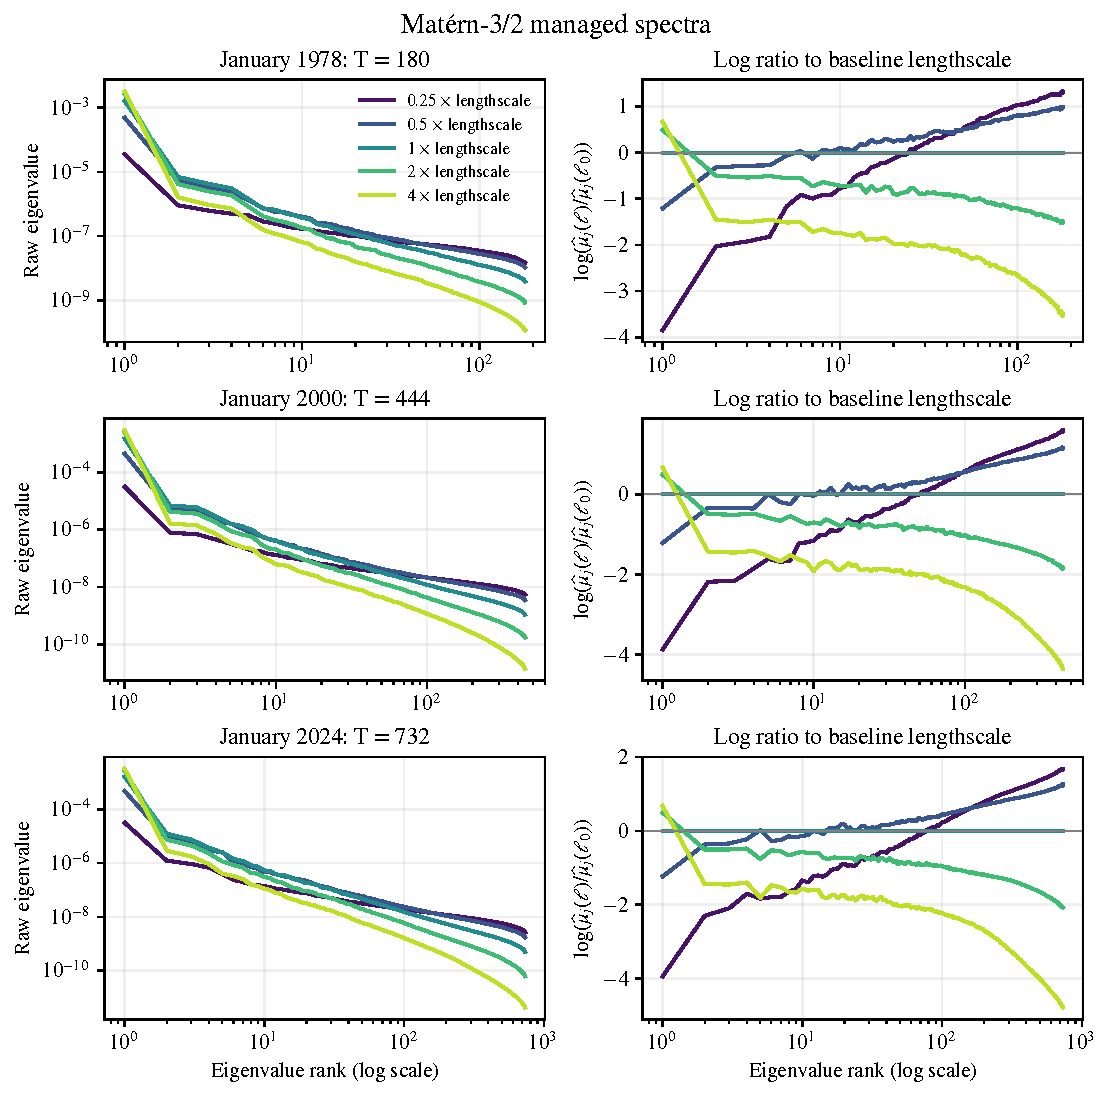
\includegraphics[width=\linewidth,height=.76\textheight,keepaspectratio]{../figures/figure1_spectral_shape.pdf}\end{center}
All five Matérn lengths use identical expanding observations. A pure amplitude change would give horizontal log-ratio curves. Leading, middle and sample-tail ratios differ. These finite-rank sample spectra do not identify a population exponent.

\newpage
\section*{Amplitude and exponent sensitivity}
\begin{center}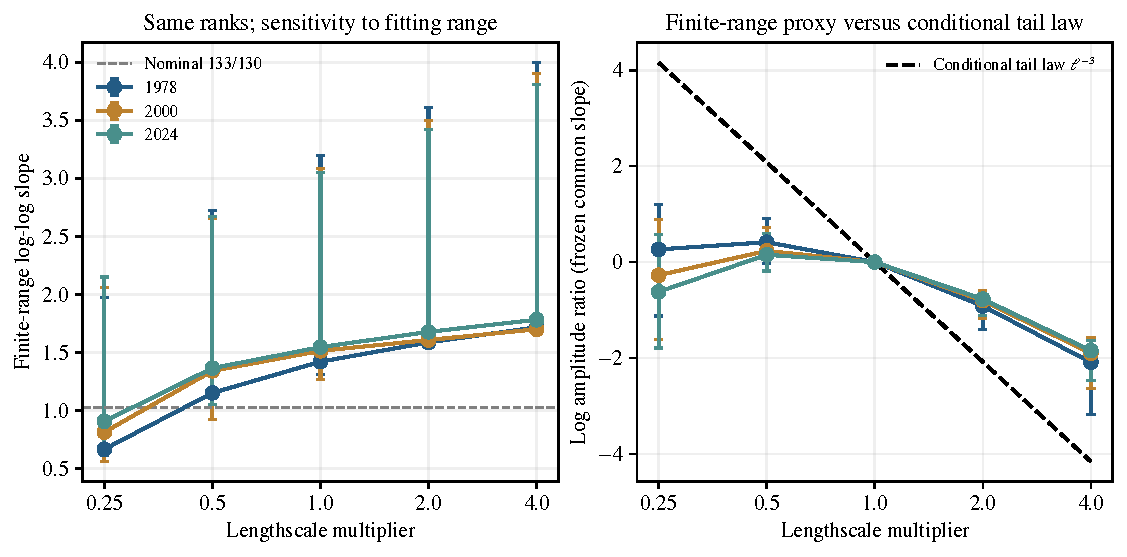
\includegraphics[width=\linewidth,height=.76\textheight,keepaspectratio]{../figures/figure2_amplitude_exponent.pdf}\end{center}
Points use ranks 11--60; whiskers span the six predeclared rank intervals. They show fit sensitivity, not confidence intervals for population b or c. The dashed amplitude law requires additional Weyl and return-covariance assumptions. A high R-squared does not establish common slope or amplitude identification.

\newpage
\section*{Predicted and selected penalties}
\begin{center}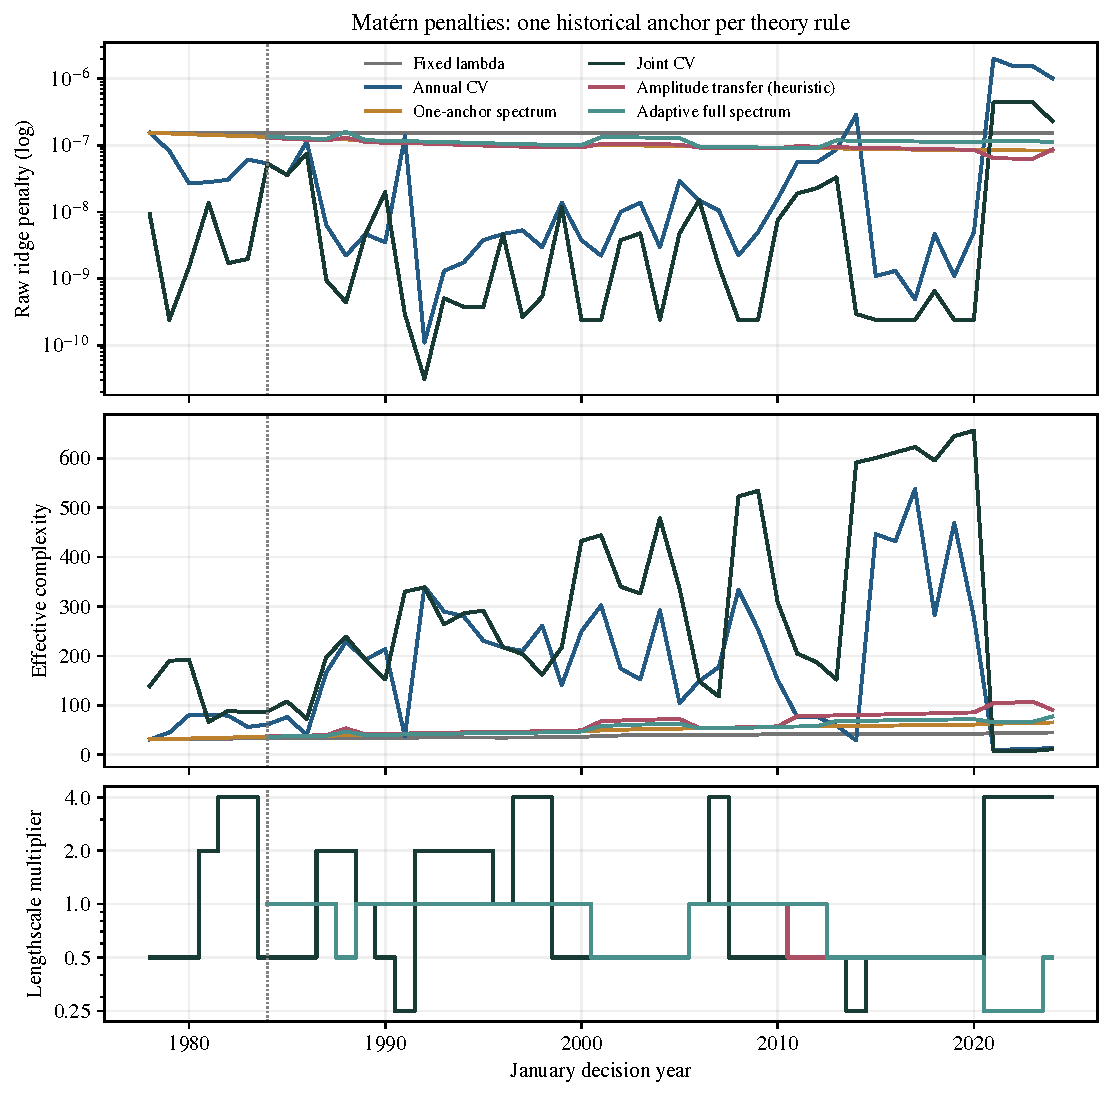
\includegraphics[width=\linewidth,height=.76\textheight,keepaspectratio]{../figures/figure3_penalty_complexity.pdf}\end{center}
Transfer uses one baseline historical anchor, a frozen finite-range b and a robust c proxy. Spectral roots use the full past empirical spectrum. Bounds are never expanded after outcomes. Adaptive paths begin in 1984; a smoother complexity trajectory is not proof of economic value.

\newpage
\section*{Financial performance and paired uncertainty}
\begin{center}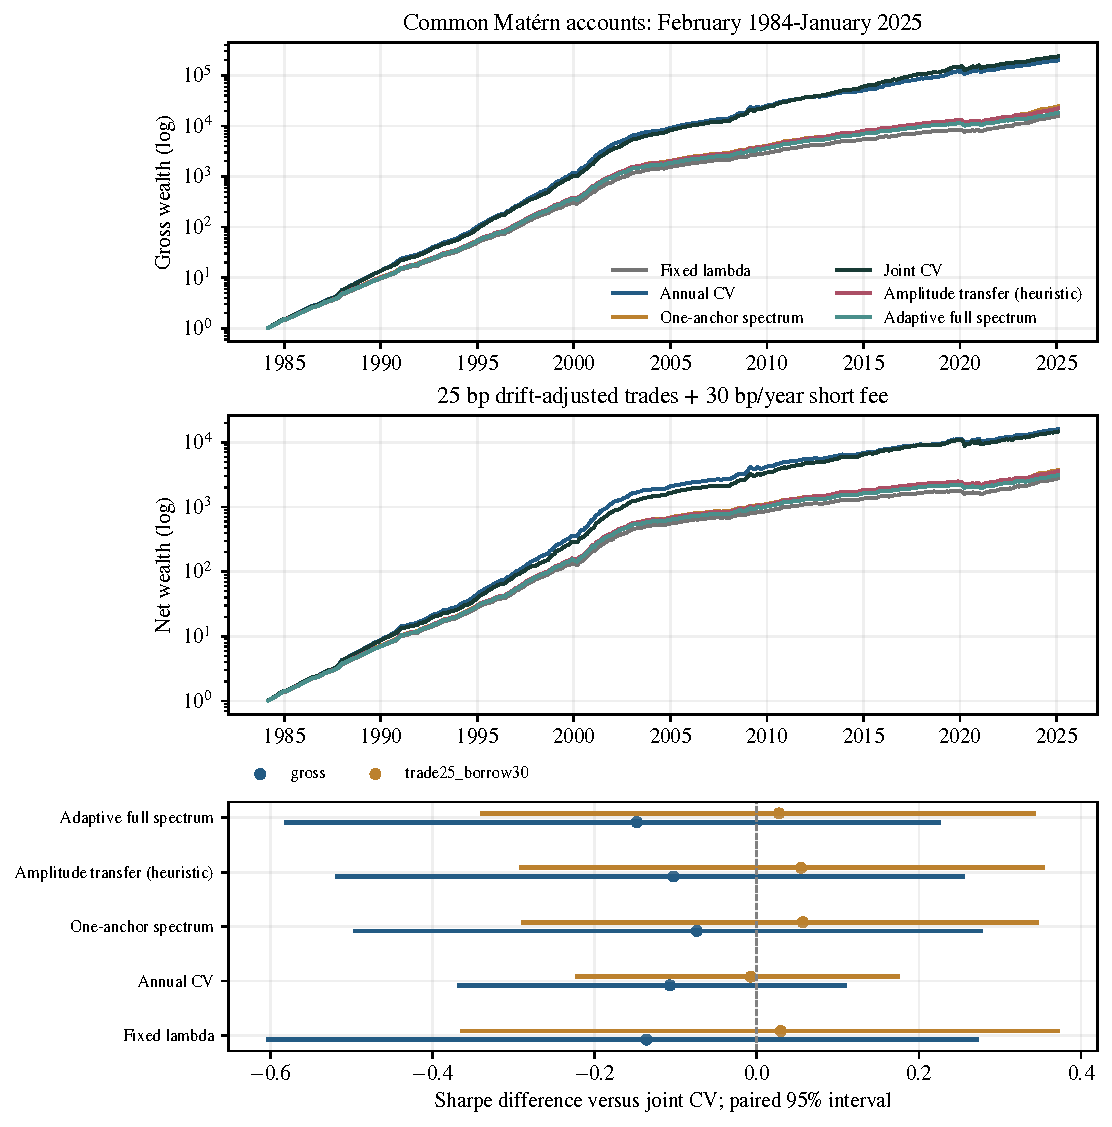
\includegraphics[width=\linewidth,height=.76\textheight,keepaspectratio]{../figures/figure4_financial_results.pdf}\end{center}
Accounts are normalized at the common start. Exact net is reconstructed from each policy's signed weights. The final panel compares Sharpe to joint CV with 12-month circular blocks and 5,000 shared draws. Six- and 24-month intervals and subperiods are retained rather than selecting a favorable sensitivity.
\newpage\section*{Requested Gaussian transfer extension}
\begin{center}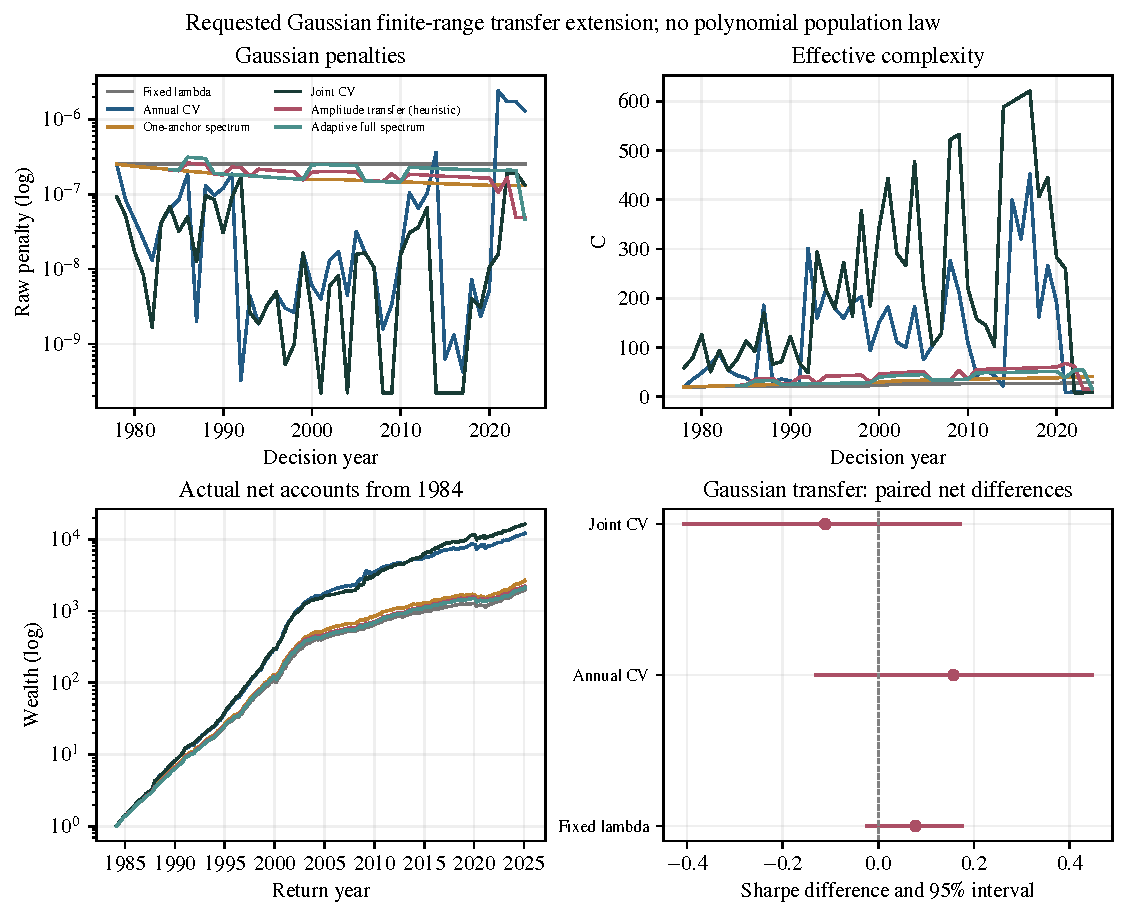
\includegraphics[width=\linewidth,height=.7\textheight,keepaspectratio]{../figures/appendix_gaussian_transfer.pdf}\end{center}
The same one-anchor transfer pipeline is applied to Gaussian with its own frozen 1978 finite-range slope 1.6234. This amendment was requested after the initial Matérn-primary run; all rank ranges, dates, bounds and candidate-selection windows remain fixed. Gaussian decay speed can change with lengthscale. The local power-law fit
is therefore a falsifiable finite-range surrogate, not a population spectral theorem.
All six primary controls have actual stock-level net accounting on the same 492 months.
\newpage\section*{Falsification, controls and costs}
Original-grid ex-post loss minima and Sharpe maxima are hindsight diagnostics only.
They never enter calibration or portfolio decisions and are not population oracles.
The following log-penalty prediction RMSEs cover the five lengths and decisions
1984--2024; small error to historical CV is not itself an investment gain.
\begin{center}\small\begin{tabular}{lrr}\toprule
Matérn rule & RMSE to CV & RMSE to hindsight loss grid\\\midrule
fixed\_lambda & 4.426 & 5.106\\
spectral & 4.029 & 4.724\\
transfer & 3.892 & 4.607\\
transfer\_nominal & 3.937 & 4.651\\
transfer\_adjusted & 3.464 & 4.226\\
\bottomrule\end{tabular}\end{center}
Matérn joint versus fixed-length CV gross Sharpe changes by +0.107; symmetric representation/penalty contrasts are +0.115/-0.008, with interaction +0.173. The amplitude-predicted cross-length shift has log-effect RMSE 2.309 to CV and 0.267 to full-spectrum shifts.
The two crossed lengthscale/penalty policies hold one component fixed at a time.
They distinguish observed representation and shrinkage contributions, but selected
hyperparameters interact, so no causal decomposition is claimed. The fixed-length
transfer control and the fixed-lambda control show whether updating spectra adds
value without changing representation. The adjusted transfer consumes five first-year
CV choices and is a separate extra-information method, not a recovered structural ratio.

The extra 1978 CV anchor at multiplier 0.25 is on a boundary in both kernels.
Adjusted transfer uses the FOC interval endpoint: a lower-bound anchor permits
$0<\rho\leq T/S(\lambda_{\min})$, and an upper-bound anchor permits
$\rho\geq T/S(\lambda_{\max})$. It does not identify a unique ratio.
\section*{Actual accounting and robustness}
Every primary method's stock weights reconstruct its managed payoff. Original CV
weights and full-history net accounts reconcile. All common-window accounts charge
entry from cash together in 1984; terminal holdings are marked without forced
liquidation. Target-weight-turnover subtraction is a separate exported scenario.
No transaction cost is borrowed from another portfolio. Illustrative fees do not
include observed execution impact, lending availability or extra funding spreads.
Predeclared history lengths, normalized feature prefixes and numerical rank thresholds
quantify finite-sample sensitivity. The Gaussian appendix is a negative control;
its population spectrum is not assigned a polynomial exponent. The requested
Gaussian finite-range transfer is an exploratory falsification exercise.
\newpage\section*{Decision and scientific limits}
\textbf{Does adaptive theory-guided shrinkage beat fixed lambda?} Matérn amplitude-transfer net Sharpe difference versus fixed lambda is +0.025 [-0.060, +0.107]; adaptive full-spectrum difference is -0.002 [-0.083, +0.067]. These paired intervals, with 6/24-month sensitivities, determine the strength of evidence. A small point difference is not a demonstrated financial gain.

\textbf{Does it beat annual CV?} Matérn transfer net difference is +0.062 [-0.184, +0.300]; adaptive full spectrum is +0.035 [-0.221, +0.281]. All methods share February 1984-January 2025 and all primary net accounts enter from cash together.

\textbf{Does it beat joint CV?} Matérn transfer net difference is +0.055 [-0.290, +0.352]; adaptive full spectrum is +0.027 [-0.338, +0.342]. Joint CV is the strongest pre-existing practical benchmark; selecting five theory-guided candidates from trailing returns remains hyperparameter selection.

\textbf{Can B(ell)/A(ell) be treated as constant?} It is a tested hypothesis, not established by RKHS equivalence. Historical per-lengthscale CV-implied FOC ratios vary, and source/score geometry changes with the RKHS norm. The additional five-anchor adjusted rule is explicitly separate; it consumes extra validation information and cannot identify a unique structural bound constant.

\textbf{Is there a defensible one-page contribution for the paper?} NO-GO. The conditional spectral-order/transfer proposition and the signal/noise counterexample are defensible mathematics, but they do not establish a useful one-constant oracle formula for this experiment. A separate one-page candidate records the negative diagnostic; do not insert it or expand the manuscript without approval.

The mathematical note proves a conditional norm/order comparison and an
asymptotic bound-proxy transfer formula, and provides a same-spectrum/different-risk-oracle
counterexample. Ordinary kernel spectra and managed-return spectra are distinct.
Two-sided polynomial bounds need not identify an asymptotic constant. Neither
fixed-penalty bounds nor smooth empirical paths establish data-dependent oracle
optimality, structural rho, or a polynomial Gaussian law. The full decision memo
answers every requested scientific question; all negative and inconclusive results,
paired sensitivities, tables, tests and input/source hashes are retained.
\end{document}
